\documentclass[tikz,border=10pt]{standalone}
\usepackage{tikz}

\begin{document}
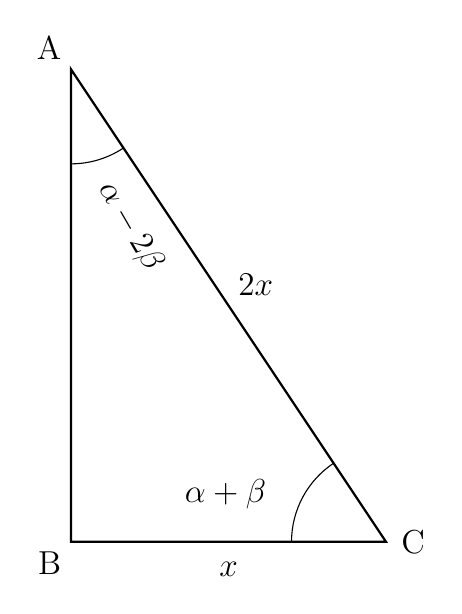
\begin{tikzpicture}[scale=1, every node/.style={font=\large}] % Set global font size to large

    % --- Coordinates ---
    % Defining points for a right-angled triangle ABC
    \coordinate (B) at (0,0);
    \coordinate (C) at (4,0); 
    \coordinate (A) at (0,6); 

    % --- Lines ---
    % Draw the triangle sides: AB, BC, and the hypotenuse AC
    \draw[thick] (A) -- (B) -- (C) -- cycle;

    % --- Arcs for Angles ---
    % Angle at A: alpha - 2*beta
    \draw (0,4.8) arc (-90:-56.3:1.2);
    
    % Angle at C: alpha + beta
    \draw (2.8,0) arc (180:123.7:1.2);

    % --- Labels and Measurements ---
    % Point Labels
    \node[above left] at (A) {A};
    \node[below left] at (B) {B};
    \node[right=2pt] at (C) {C};

    % Side Measurements
    \node[above right] at (2, 3) {$2x$}; 
    \node[below=4pt] at (2, 0) {$x$};     

    % --- Angle Labels (FIXED PLACEMENT) ---
    % Shifted to the left (0.75) and down (4.0) to avoid the hypotenuse line
    \node[rotate=-60] at (0.75, 4.0) {$\alpha-2\beta$};
    
    % Shifted slightly more to the left to clear the arc and side
    \node[left] at (2.6, 0.6) {$\alpha+\beta$};

\end{tikzpicture}
\end{document}